\documentclass[a4paper,12pt]{article}
\usepackage[lithuanian]{babel}
% \usepackage[T1]{fontenc} % Don't need this when using LuaLatex instead of PDFLatex
\usepackage{amsmath}
\usepackage{graphicx}
\usepackage{float}
\usepackage{listings}
\usepackage{xcolor}

\title{Vienmačio optimizavimo metodai}
\author{Kristupas Dansevičius}
\date{\today}

\begin{document}

\maketitle
\tableofcontents

\section{Įvadas}
Šis laboratorinis darbas paskirtas optimizavimo metodų kurse Vilniaus Universitete. 
Šiame darbe nagrinėjami trys vienmačio optimizavimo metodai:
intervalo dalijimo pusiau metodas, auksinio pjūvio metodas ir Niutono metodas.

\begin{enumerate}
    \item 
\end{enumerate}

\[
f(x) = \frac{(x^2 - 5)^2}{4}
\]

\section{Metodai}
\subsection{Intervalo dalijimo pusiau metodas}
Tai tritaškis intervalo dalijimo pusiau metodas, kurio principas yra itin paprastas:
intervale panaudojami 3 taškai:
\begin{itemize}
    \item $x_{middle}$ - tai vidurinis taškas esantis intervalo viduryje
    \item $x_1$ - tai viduryje tarp kairiojo intervalo krašto ir vidurinio taško $x_{middle}$ esantis taškas
    \item 
\end{itemize}

\subsection{Auksinio pjūvio metodas}
Trumpas metodo aprašymas.

\subsection{Niutono metodas}
Trumpas metodo aprašymas.

\section{Rezultatai}
Gauti šie rezultatai:

\begin{itemize}
    \item Intervalo dalijimo pusiau metodas: 
        $x_{\min} \approx 2.236$, iteracijų: 17, funkcijos iškvietimų: 28
    \item Auksinio pjūvio metodas:
        $x_{\min} \approx 2.236$, iteracijų: 24, funkcijos iškvietimų: 26
    \item Niutono metodas:
        $x_{\min} \approx 2.236$, iteracijų: 6, funkcijos iškvietimų: 12
\end{itemize}

\section{Vizualizacija}
Žemiau pateikiamos tikslo funkcijos ir taikytų metodų vizualizacijos.

\begin{figure}[H]
    \centering
    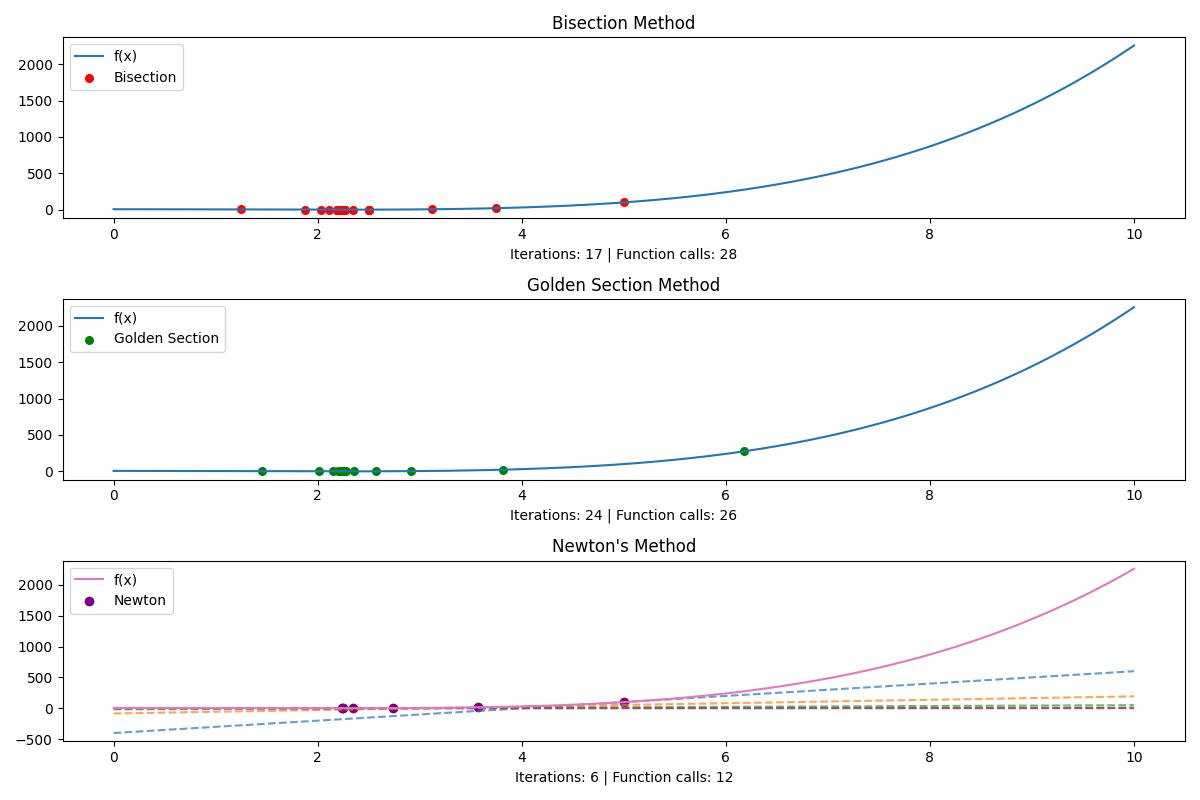
\includegraphics[width=\textwidth]{figure-1.jpeg}
    \caption{\label{fig:all}Funkcijos $f(x)$ optimizavimo vizualizacija.}
\end{figure}

\section{Išvados}
\begin{itemize}
    \item Visi metodai rado minimumą ties $x \approx \sqrt{5}$.
    \item Intervalo metodai reikalauja daugiau iteracijų, bet yra paprastesni.
    \item Niutono metodas greitesnis, bet priklausomas nuo pradinio taško.
\end{itemize}

\section{Kodas}
\lstinputlisting[language=python]{../code/main.py}
\end{document}